\title{Lecture 6\\Representation of Relations and Their Properties in a Knowledge Base}

\begin{frame}
	\titlepage
\end{frame}

\begin{frame}{\\Lecture outline}
	\topline
	\justifying
	Binary relations and ways of specifying them. Reflexive and irreflexive binary relations. Symmetric and antisymmetric binary relations. Transitive binary relations. Strict and non-strict order relations. Total (linear) and partial order relations. Equivalence and tolerance relations. Quasi-binary relations. n-ary relations and relation schemas. Domain of definition and attribute domains. Operations on relations (projection, join, composition). Metarelations and examples. Representation in a knowledge base.
\end{frame}

\begin{frame}{\\The concept of a relation}
	\topline
	\justifying

	A \textbf{\textit{relation}} is understood as a subset of a Cartesian power of a set.\\

	\textbf{\textit{A relation}}, \textit{defined on a set M} is a subset of the \textit{Cartesian product} of that set with itself a certain number of times.\\

	\scnheader{relation}
	\scnrelfrom{illustration}{
		\begin{center}
			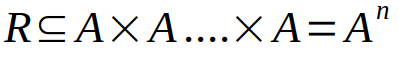
\includegraphics[width=35mm]{figures/sd_sets/relative.png}

		\end{center}
	}

	In a broader sense, a {\textbf{\textit{relation}}} is a mathematical structure that formally defines the properties of objects and their interconnections.
\end{frame}

\begin{frame}{\\Specifying relations}



	\topline
	\justifying

	Relation theory uses the following main representations of binary relations.\\

	\begin{textitemize}
		\item \textit{Enumeration of elements}. A relation R between elements of sets A and B is specified by listing the pairs belonging to R.

		\item
		\textit{Matrix representation}. A binary relation is represented by a \textit{Boolean} (binary) matrix.

		\item \textit{Graphical representation}. A binary relation is represented graphically by a directed bipartite graph.

	\end{textitemize}

\end{frame}

\begin{frame}{\\Classification of relations}

	\topline
	\justifying
	\footnotesize

	\begin{SCn}
		\scnheader{relation}

		\begin{scnrelfromset}{partition}
			\scnitem{class of equicardinal tuples}
			\scnitem{class of tuples of different cardinalities}
		\end{scnrelfromset}

		\begin{scnrelfromset}{partition}
			\scnitem{binary relation}
			\scnitem{non-binary relation}
		\end{scnrelfromset}

		\begin{scnrelfromset}{partition}
			\scnitem{directed relation}
			\scnitem{undirected relation}
		\end{scnrelfromset}

		\begin{scnrelfromset}{partition}
			\scnitem{role relation}
			\scnitem{non-role relation}
		\end{scnrelfromset}

	\end{SCn}
\vspace{-2em}
\end{frame}

\begin{frame}{\\Class of equicardinal tuples}

	\topline
	\justifying

	\begin{SCn}
		\scnheader{class of equicardinal tuples}
		\scnidtf{class of tuples of fixed arity}
		\scnidtf{relation with the property of arity}
		\scnsuperset{unary relation}
		\scnsuperset{binary relation}
		\scnsuperset{ternary relation}
		\scntext{definition}{\textbf{\textit{class of equicardinal tuples}} is a class of tuples with the same cardinality.}
	\end{SCn}

\end{frame}

\begin{frame}{\\Class of tuples of different cardinalities}

	\topline
	\justifying

	\begin{SCn}
		\scnheader{class of tuples of different cardinalities}
		\scnidtf{relation of variable arity}
		\scnsubset{non-binary relation}
		\scntext{definition}{\textbf{\textit{class of tuples of different cardinalities}} is a class of tuples with different cardinalities.}
	\end{SCn}
\end{frame}

\begin{frame}{\\Unary relation}%
	\topline
	\justifying
	\begin{SCn}
		\scnheader{unary relation}
		\scnidtf{relation of arity one}
		\scnidtf{one-place set}
		\scnidtf{set of singletons}
		\scntext{definition}{\textbf{\textit{unary relation}} is a set of relations on a set M that are arbitrary subsets of M.}
	\end{SCn}
\end{frame}

\begin{frame}{\\Binary relation}%
	\topline
	\justifying
	\begin{SCn}
		\scnheader{binary relation}
		\scnidtf{relation of arity two}
		\scnidtf{two-place relation}
		\scnsuperset{quasi-binary relation}
		\scnsuperset{order relation}
		\scnsuperset{tolerance relation}
		\begin{scnrelfromset}{partition}
			\scnitem{reflexive relation}
			\scnitem{irreflexive relation}
			\scnitem{partially reflexive relation}
		\end{scnrelfromset}
		\begin{scnrelfromset}{partition}
			\scnitem{symmetric relation}
			\scnitem{antisymmetric relation}
			\scnitem{partially symmetric relation}
		\end{scnrelfromset}
	\end{SCn}
\vspace{-2em}
\end{frame}

\begin{frame}%
	\begin{SCn}
		\scnheader{binary relation}
		\begin{scnrelfromset}{partition}
			\scnitem{transitive relation}
			\scnitem{antitransitive relation}
			\scnitem{partially transitive relation}
		\end{scnrelfromset}
		\begin{scnrelfromset}{partition}
			\scnitem{role relation}
			\scnitem{non-role relation}
		\end{scnrelfromset}
	\end{SCn}
\scntext{definition}{\textbf{\textit{binary relation}} is a set of relations on a set \textbf{\textit{M}} that are subsets of the \textit{ Cartesian product} set \textbf{\textit{M}}.\\
If a \textbf{\textit{binary relation R}} is defined on a \textit{set \textbf{M}} and two elements of this set \textbf{\textit{a}} and \textbf{\textit{b}} are related by it, we denote this connection by \textbf{\textit{aRb}}.}
\end{frame}

\begin{frame}{\\Quasi-binary relation}%

	\topline
	\justifying

	\scnheader{quasi-binary relation}
	\scntext{explanation}{ \textbf{\textit{quasi-binary relation}} is a set of ordered pairs in which at least one component is a tuple.\\
Thus, \textit{sc-arcs} belonging to \textbf{\textit{quasi-binary relations}} always originate from or terminate at a tuple.}
	\scnhaselement{partition*}
	\scnhaselement{intersection*}
	\scnhaselement{union*}

\vspace{-2em}
\end{frame}

\begin{frame}{\\Non-binary relation}%
	\topline
	\justifying
	\scnheader{non-binary relation}
	\scntext{explanation}{\textbf{\textit{non-binary relation}} is a set of relations each of which has at least one tuple with cardinality greater than two.}
	\end{frame}

\begin{frame}{\\Directionality of relations}%
	\topline
	\justifying
	\scnheader{directed relation}
	\scntext{definition}{\textbf{\textit{directed relation}} is a set of relations each of whose tuples is an ordered tuple.}
	\scnheader{undirected relation}
	\scntext{definition}{\textbf{\textit{undirected relation}} is a set of relations each of whose tuples is an unordered set.}
	\end{frame}



\begin{frame}{\\Properties of binary relations}
	\topline
	\justifying
	\footnotesize
	\vspace{10mm}

	\scnheader{reflexive relation}
	\scntext{definition}{\textbf{\textit{reflexive relation}} on \textit{set {\textbf{A}}} is a \textit{binary relation} in which every element of the set \textbf{\textit{A}} is related by \textbf{\textit{R}} to itself.}
	\scnhaselement{equality*}

	\scnheader{irreflexive relation}
	\scntext{definition}{\textbf{\textit{irreflexive relation R}} on \textit{set {\textbf{A}}} is a \textit{binary relation} in which every element of the set \textbf{\textit{A}} is not related by \textbf{\textit{R}} to itself.}
	\scnhaselement{greater than*}
	\scnhaselement{above*}

	\scnheader{partially reflexive relation}
	\scntext{definition}{\textbf{\textit{partially reflexive relation R}} on \textit{set {\textbf{A}}} is a \textit{binary relation} in which at least one (but not all) element of the set \textbf{\textit{A}} is related by \textbf{\textit{R}} to itself.}
	\end{frame}

\begin{frame}{\\Properties of binary relations}
	\topline
	\justifying
	\scriptsize
	\vspace{10mm}

	\justifying
	\scnheader{symmetric relation}
	\scntext{definition}{\textbf{\textit{symmetric relation R}} on \textit{set {\textbf{A}}} is a \textit{binary relation} in which, for every pair of elements \textbf{\textit{a}} and \textbf{\textit{b}} of that set, the relations \textbf{\textit{aRb}} imply \textbf{\textit{bRa}}.}
	\scnhaselement{parallelism*}
	\scnhaselement{perpendicularity*}
	\scnhaselement{relative*}

	\scnheader{antisymmetric relation}
	\scntext{definition}{\textbf{\textit{antisymmetric relation R}} on \textit{set {\textbf{A}}} is a \textit{binary relation} in which, for every pair of elements \textbf{\textit{a}} and \textbf{\textit{b}} of that set, the relations \textbf{\textit{aRb}} and \textbf{\textit{bRa}} imply equality of \textbf{\textit{a}} and \textbf{\textit{b}}.}
	\scnhaselement{greater than*}
	\scnhaselement{above*}

	\scnheader{partially symmetric relation}
	\scntext{definition}{\textbf{\textit{partially symmetric relation R}} on \textit{set {\textbf{A}}} is a \textit{binary relation} in which, for every pair of elements \textbf{\textit{a}} and \textbf{\textit{b}} (but not for all such pairs) of that set, the relations \textbf{\textit{aRb}} imply \textbf{\textit{bRa}}.}
	\end{frame}

\begin{frame}{\\Properties of binary relations}
	\topline
	\justifying
	\scriptsize
	\vspace{10mm}

	\justifying
	\scnheader{transitive relation}
	\scntext{definition}{\textbf{\textit{transitive relation R}} on \textit{set {\textbf{A}}} is a \textit{binary relation} in which, for any three elements of that set \textbf{\textit{a}}, \textbf{\textit{b}}, \textbf{\textit{c}} the relations \textbf{\textit{aRb}} and \textbf{\textit{bRc}} imply the relation \textbf{\textit{aRc}}.}
	\scnhaselement{parallelism*}
	\scnhaselement{relative*}

	\scnheader{antitransitive relation}
	\scntext{definition}{\textbf{\textit{antitransitive relation R}} on \textit{set {\textbf{A}}} is a \textit{binary relation} in which, for any three elements of that set \textbf{\textit{a}}, \textbf{\textit{b}}, \textbf{\textit{c}} the relations \textbf{\textit{aRb}} and \textbf{\textit{bRc}} do not imply the relation \textbf{\textit{aRc}}.}
	\scnhaselement{perpendicularity*}

	\scnheader{partially transitive relation}
	\scntext{definition}{\textbf{\textit{partially transitive relation R}} on \textit{set {\textbf{A}}} is a \textit{binary relation} in which, for every three elements of that set \textbf{\textit{a}}, \textbf{\textit{b}}, \textbf{\textit{c}} (but not for all such triples), the relations \textbf{\textit{aRb}} and \textbf{\textit{bRc}} imply the relation \textbf{\textit{aRc}}.}

\end{frame}

\begin{frame}{\\Order relation}%
	\topline
	\justifying
	\begin{SCn}
		\scnheader{order relation}
		\begin{scnrelfromset}{partition}
			\scnitem{strict order relation}
			\scnitem{non-strict order relation}
			\end{scnrelfromset}
		\begin{scnrelfromset}{partition}
			\scnitem{total order relation}
			\scnitem{partial order relation}
			\end{scnrelfromset}
		\end{SCn}
	\scntext{definition}{\textbf{\textit{order relation}} is a \textit{binary relation} with the properties of transitivity and antisymmetry.}
\end{frame}

\begin{frame}{\\Strict and non-strict order relations}%
\topline
\justifying
	\scnheader{strict order relation}
	\scntext{definition}{\textbf{\textit{strict order relation}} is a \textit{order relation} with the property of irreflexivity.}
	\scnhaselement{greater than*}

	\scnheader{non-strict order relation}
	\scntext{definition}{\textbf{\textit{non-strict order relation}} is a \textit{order relation} with the property of reflexivity.}
	\scnhaselement{greater than or equal to*}

	\end{frame}

\begin{frame}{\\Tolerance relation}%
	\topline
	\justifying
	\scnheader{tolerance relation}
	\scntext{definition}{\textbf{\textit{tolerance relation}} is a \textit{binary relation} belonging to the classes of \textit{symmetric relation} and \textit{reflexive relation}.}
	\end{frame}

\begin{frame}{\\Equivalence relation}%
	\topline
	\justifying
	\begin{SCn}
		\scnheader{equivalence relation}
		\scnidtf{maximal family of equivalence relations}
		\scnsubset{tolerance relation}
		\scnhaselement{equality*}
		\scntext{definition}{\textbf{\textit{equivalence relation}} is a \textit{tolerance relation} belonging to the class of \textit{transitive relations}}
		\scntext{note}{Each equivalence relation specifies what we consider equivalent entities: which similarities we focus on and which differences we ignore.}
	\end{SCn}
\end{frame}

\begin{frame}{\\Role relation}%
	\topline
	\justifying
	\begin{SCn}
		\scnheader{role relation}
		\scnidtf{attribute}
		\scnidtf{attributive relation}
		\scnidtf{relation specifying the role of elements within a set}
		\scnidtf{relation that is a subset of the membership relation}
		\scnrelto{family of subsets}{membership*}
		\scnsubset{binary relation}
		\scnsuperset{numerical attribute}

		\scntext{explanation}{\textbf{\textit{role relation}} is a relation that is a subset of the membership relation.}
	\end{SCn}
\end{frame}

\begin{frame}%
	\scntext{instance identification rule}{At the end of each \textit{identifier} of an instance of the class \textbf{\textit{role relation}} that is not a system identifier, the symbol `` \scnrolesign '' is added.

For example:\\
		\textit{key instance\scnrolesign}

		Because of restrictions on the allowed alphabet, a system identifier cannot contain the symbol ``\scnrolesign''. Therefore, each \textit{system identifier} of an instance of the class \textbf{\textit{role relation}} is prefixed with ``rrel\_''.

For example:\\
		\textit{rrel\_key\_sc\_element}}
	\end{frame}

\begin{frame}{\\Numerical attribute}%
    \topline
    \justifying

	\begin{SCn}
	\scnheader{numerical attribute}
	\scnidtf{ordinal number}
	\scnidtf{component number of a directed tuple}
	\scnhaselement{\textbf{1\scnrolesign}; \textbf{2\scnrolesign}; \textbf{3\scnrolesign}; \textbf{4\scnrolesign}; \textbf{5\scnrolesign}; \textbf{6\scnrolesign}; \textbf{7\scnrolesign}; \textbf{8\scnrolesign}; \textbf{9\scnrolesign}; \textbf{10\scnrolesign}}; ...
	\scntext{explanation}{\textbf{\textit{numerical attribute}} -- \textit{role relation} that specifies the ordinal number of an element in a directed tuple without clarifying the semantics of this membership. Numerical attributes often suffice to distinguish tuple components whose semantics are specified separately, for example, in the definition of the relation to which the tuple belongs.}
	\end{SCn}
\end{frame}

\begin{frame}{\\Non-role relation}%
	\topline
	\justifying
	\begin{SCn}
		\scnheader{non-role relation}
		\begin{scnrelfromset}{partition}
		\scnitem{non-binary relation}
		\scnitem{non-role binary relation}
		\end{scnrelfromset}
		\scntext{explanation}{\textbf{\textit{non-role relation}} is a relation that is not a subset of the membership relation.}
		\end{SCn}
	\end{frame}

\begin{frame}%

		\scntext{instance identification rule}{At the end of each \textit{identifier} of an instance of the class \textbf{\textit{non-role relation}} that is not a system identifier, the symbol ``*'' is added.

For example:\\
			\textit{inclusion*}

			Because of restrictions on the allowed alphabet, a system identifier cannot contain ``*''. Therefore, each \textit{system identifier} of an instance of the class \textbf{\textit{non-role relation}} is prefixed with ``nrel\_''.

For example:\\
			\textit{nrel\_inclusion}}
		\end{frame}

\begin{frame}{\\Non-role binary relation}%
    \topline
    \justifying
	\begin{SCn}
		\scnheader{non-role binary relation}
		\scntext{explanation}{\textbf{\textit{non-role binary relation}} -- \textit{binary relation} that is not a \textit{role relation}.}
	\end{SCn}
\end{frame}

\begin{frame}{\\Arity}%
	\topline
	\justifying
	\begin{SCn}
		\scnheader{arity}
		\scnidtf{arity of a relation}
		\scniselement{parameter}
		\scntext{explanation}{\textbf{\textit{arity}} is a parameter each of whose elements is a class of \textit{relations} all of whose tuples have the same \textit{cardinality}. The value of this \textit{parameter} equals the \textit{cardinality} of each such tuple.}
	\end{SCn}
\end{frame}

\begin{frame}%
	\begin{SCn}
	\scnrelfrom{example description}{
		\begin{center}
		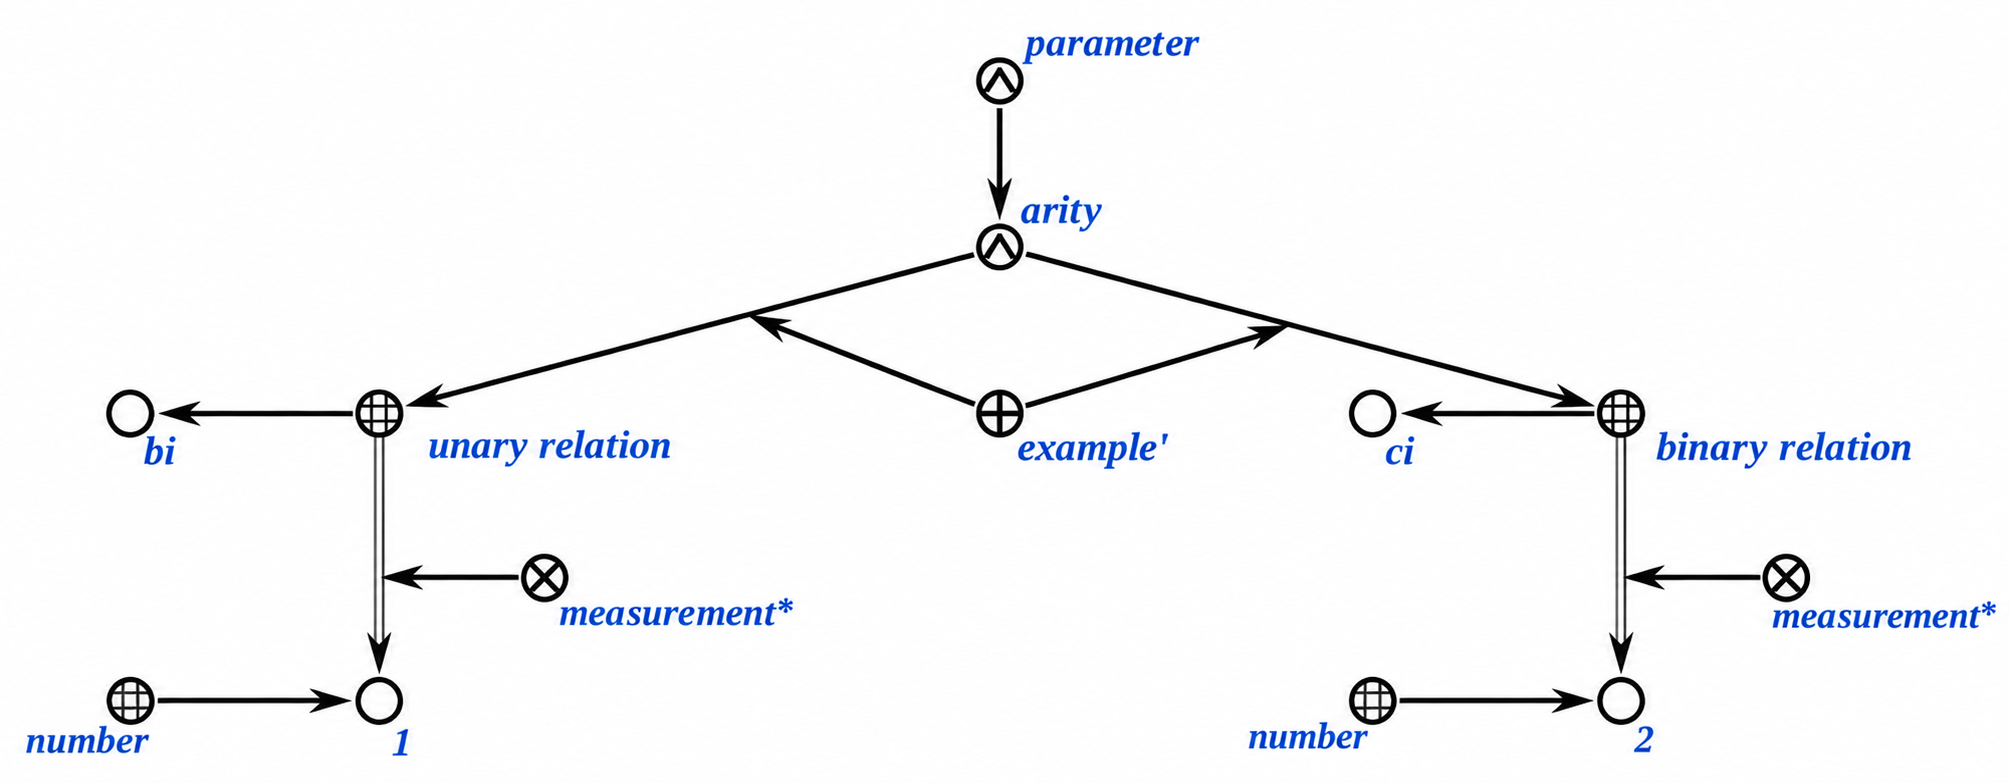
\includegraphics[width=120mm]{figures/sd_sets/arity_en.png}
	\end{center}}
\end{SCn}
\end{frame}

\begin{frame}{\\Domain of definition}%
	\topline
	\justifying
	\begin{SCn}
		\scnheader{domain of definition*}
		\scnidtf{domain of definition of a relation*}
		\scniselement{binary relation}
		\scntext{explanation}{\textbf{\textit{domain of definition*}} is a \textit{binary relation} that connects a relation to its domain of definition.

The domain of definition of a relation is the set-theoretic union of all its tuples, or equivalently, the union of all sets that are attribute domains of that relation.}
	\end{SCn}

\end{frame}

\begin{frame}%
		\begin{SCn}
		\scnrelfrom{example description}{
			\begin{center}
			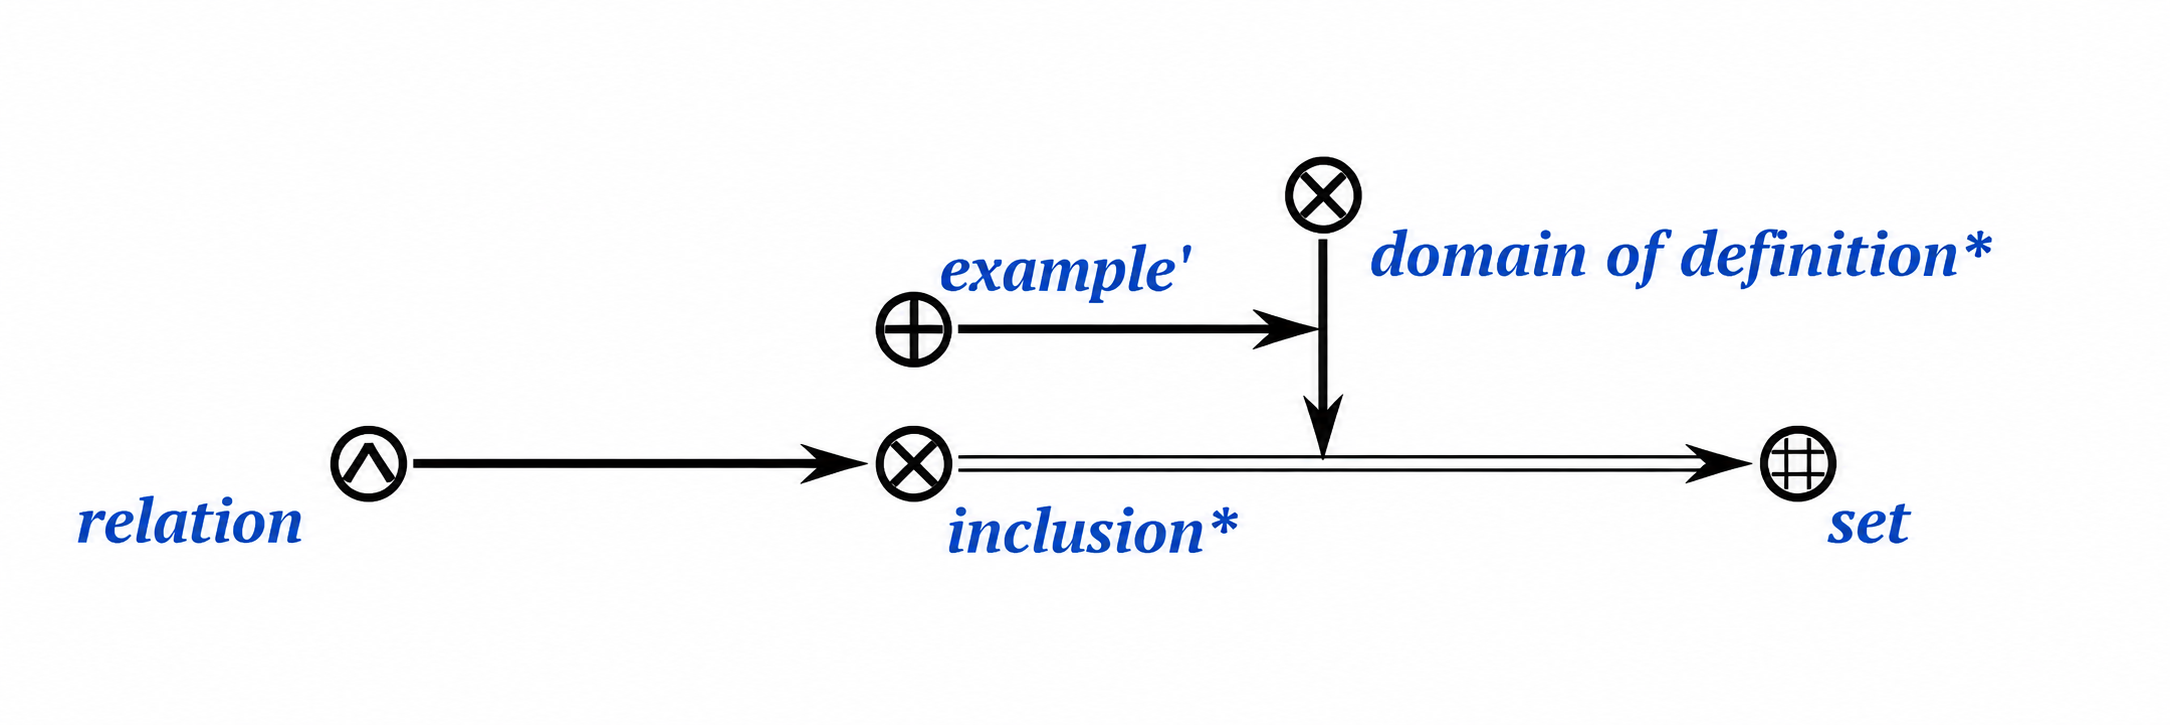
\includegraphics[width=100mm]{figures/sd_sets/domain_en.png}
		\end{center}}
	\end{SCn}
\end{frame}

\begin{frame}{\\Attribute of a relation}%
	\topline
	\justifying
	\begin{SCn}
	\scnheader{attribute of a relation*}
	\scnidtf{role attribute used in the tuples of a given relation*}
	\scniselement{binary relation}
	\scntext{explanation}{\textbf{\textit{attribute of a relation*}} is a \textit{binary relation} that connects a given relation to a \textit{role relation} used in that relation to specify the role of an element of its tuples.}
	\end{SCn}
\end{frame}

\begin{frame}%
		\scnrelfrom{example description}{
			\begin{center}
			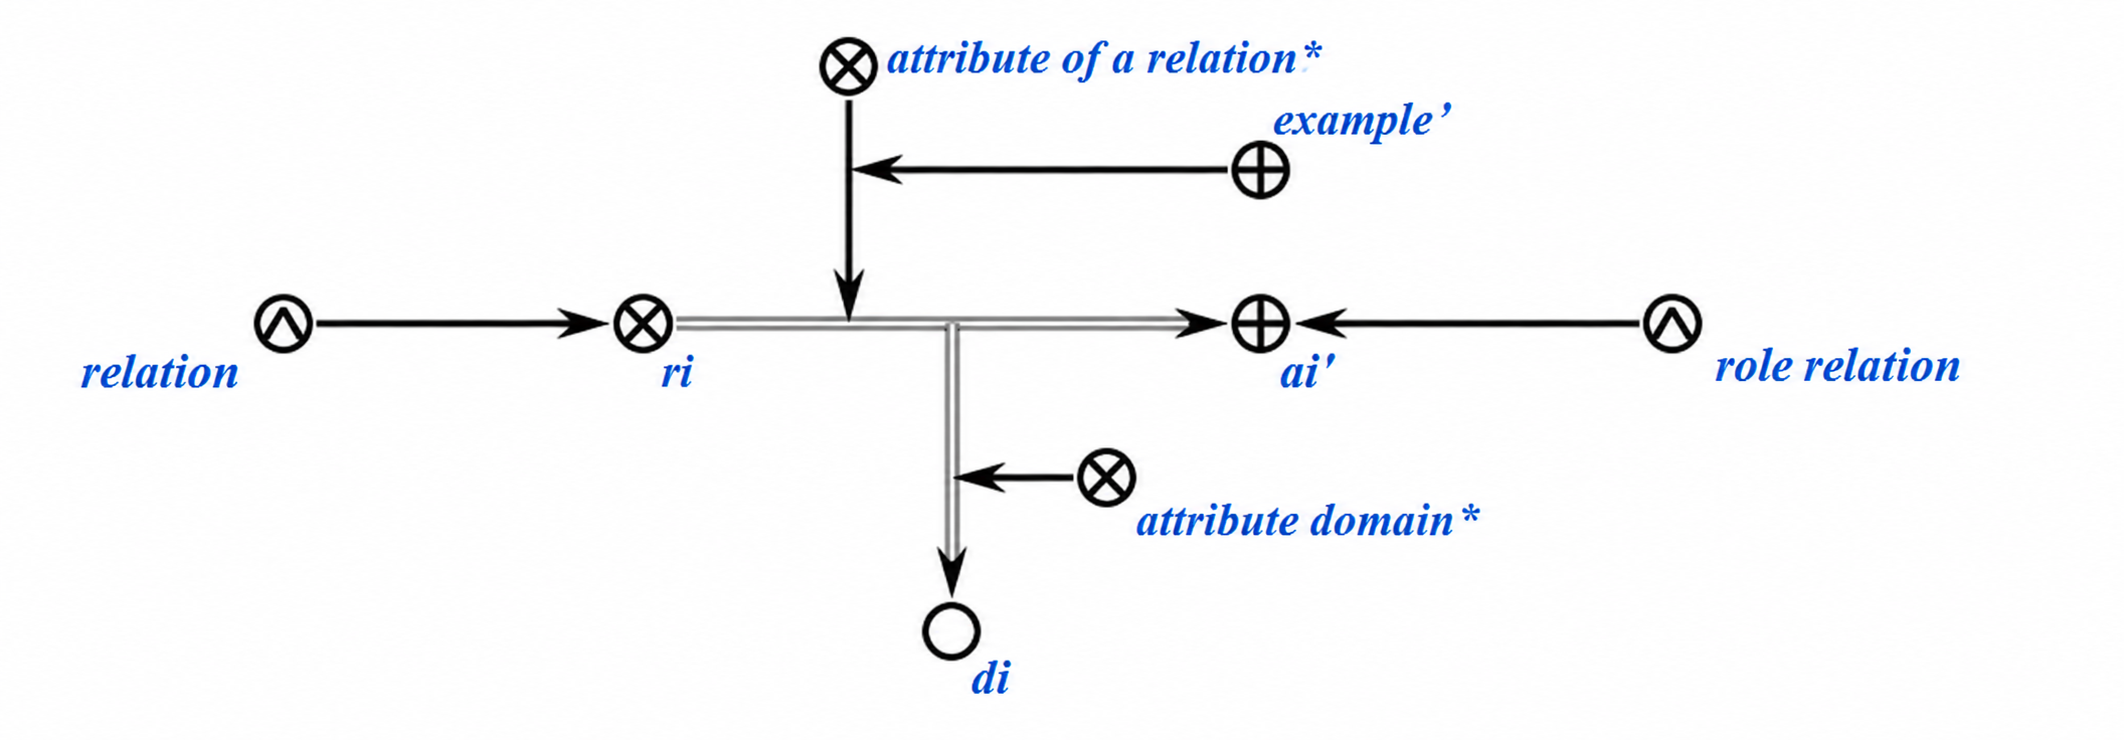
\includegraphics[width=120mm]{figures/sd_sets/relationshipAttribute_en.png}
		\end{center}}
	\end{frame}

\begin{frame}{\\Attribute domain}%
	\topline
	\justifying
	\begin{SCn}
	\scnheader{attribute domain*}
	\scnidtf{domain of a relation for a given attribute*}
	\scniselement{binary relation}
	\scntext{explanation}{\textbf{\textit{attribute domain}} is a \textit{binary relation} that connects a tuple of the relation \textit{attribute of a relation*} to the set that is the domain of a given relation for a given attribute. The set \textbf{\textit{di}} is the domain of a relation \textbf{\textit{ri}} for the attribute \textbf{\textit{ai}} if and only if the elements of that set are exactly the elements of the tuples of the relation \textbf{\textit{ri}} that have the attribute \textbf{\textit{ai}}.}
	\end{SCn}
\end{frame}

\begin{frame}%
	\scnrelfrom{example description}{
		\begin{center}
		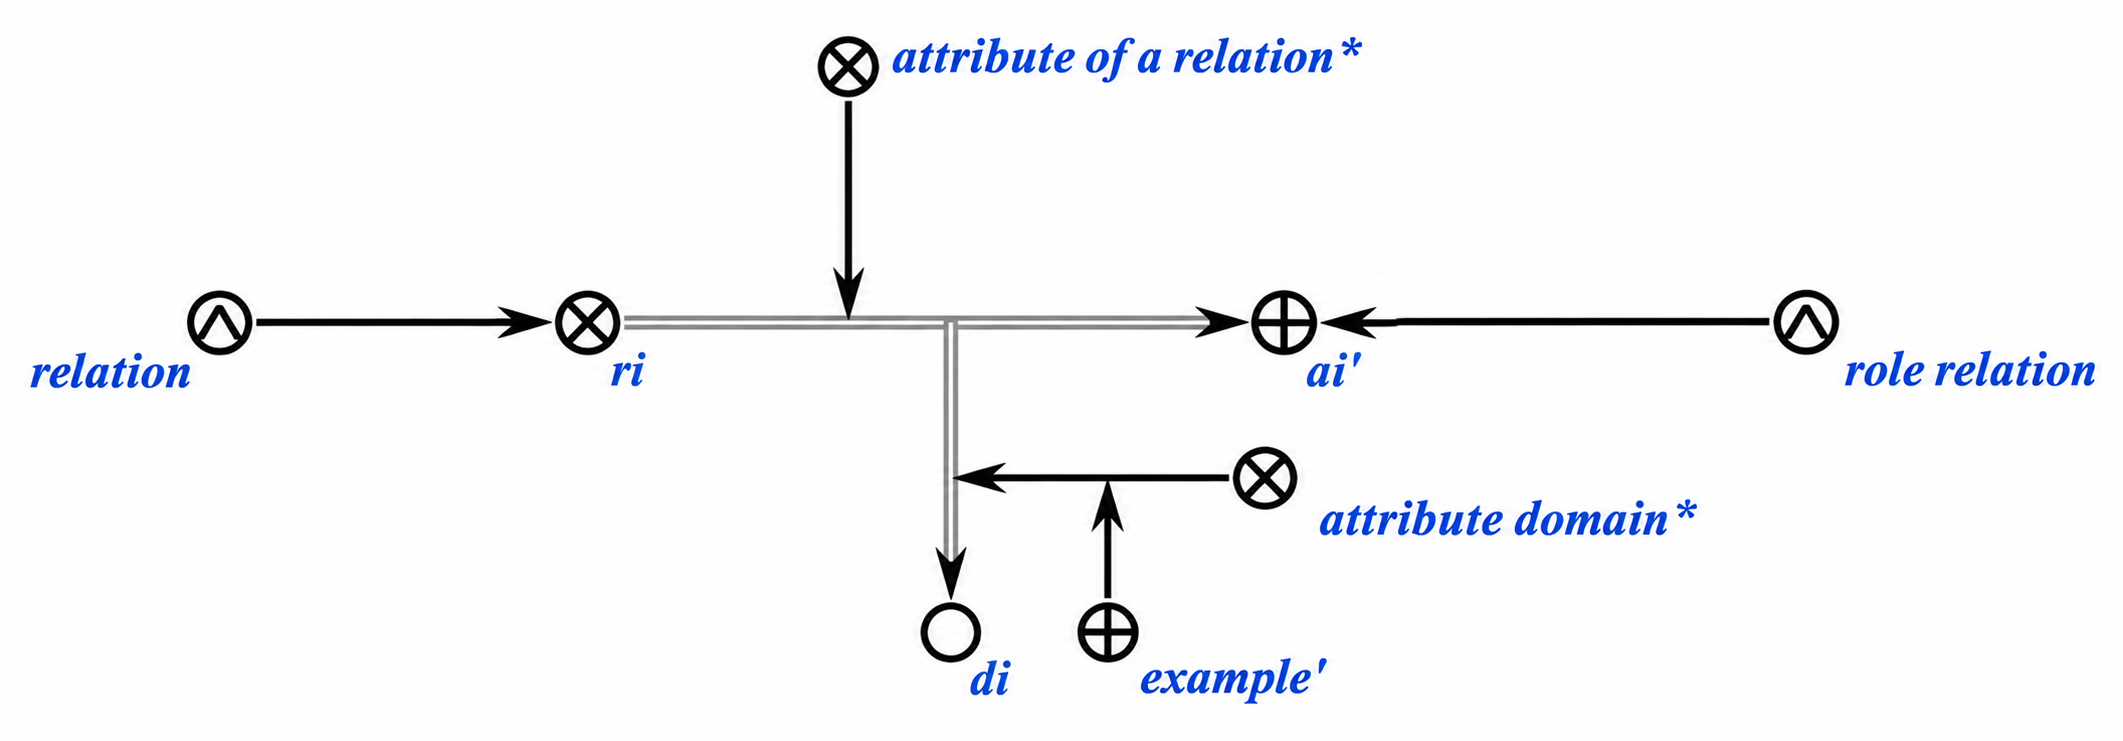
\includegraphics[width=120mm]{figures/sd_sets/domen_en.png}
	\end{center}}
\end{frame}

\begin{frame}{\\First attribute domain}%
\topline
\justifying
	\begin{SCn}
	\scnheader{first attribute domain*}
	\scniselement{binary relation}

	\scntext{definition}{\textbf{\textit{first attribute domain*}} is a \textit{binary relation} that connects a relation to its domain for the attribute \textbf{\textit {1\scnrolesign}} of that relation.}
	\scnrelfrom{example description}{
		\begin{center}
		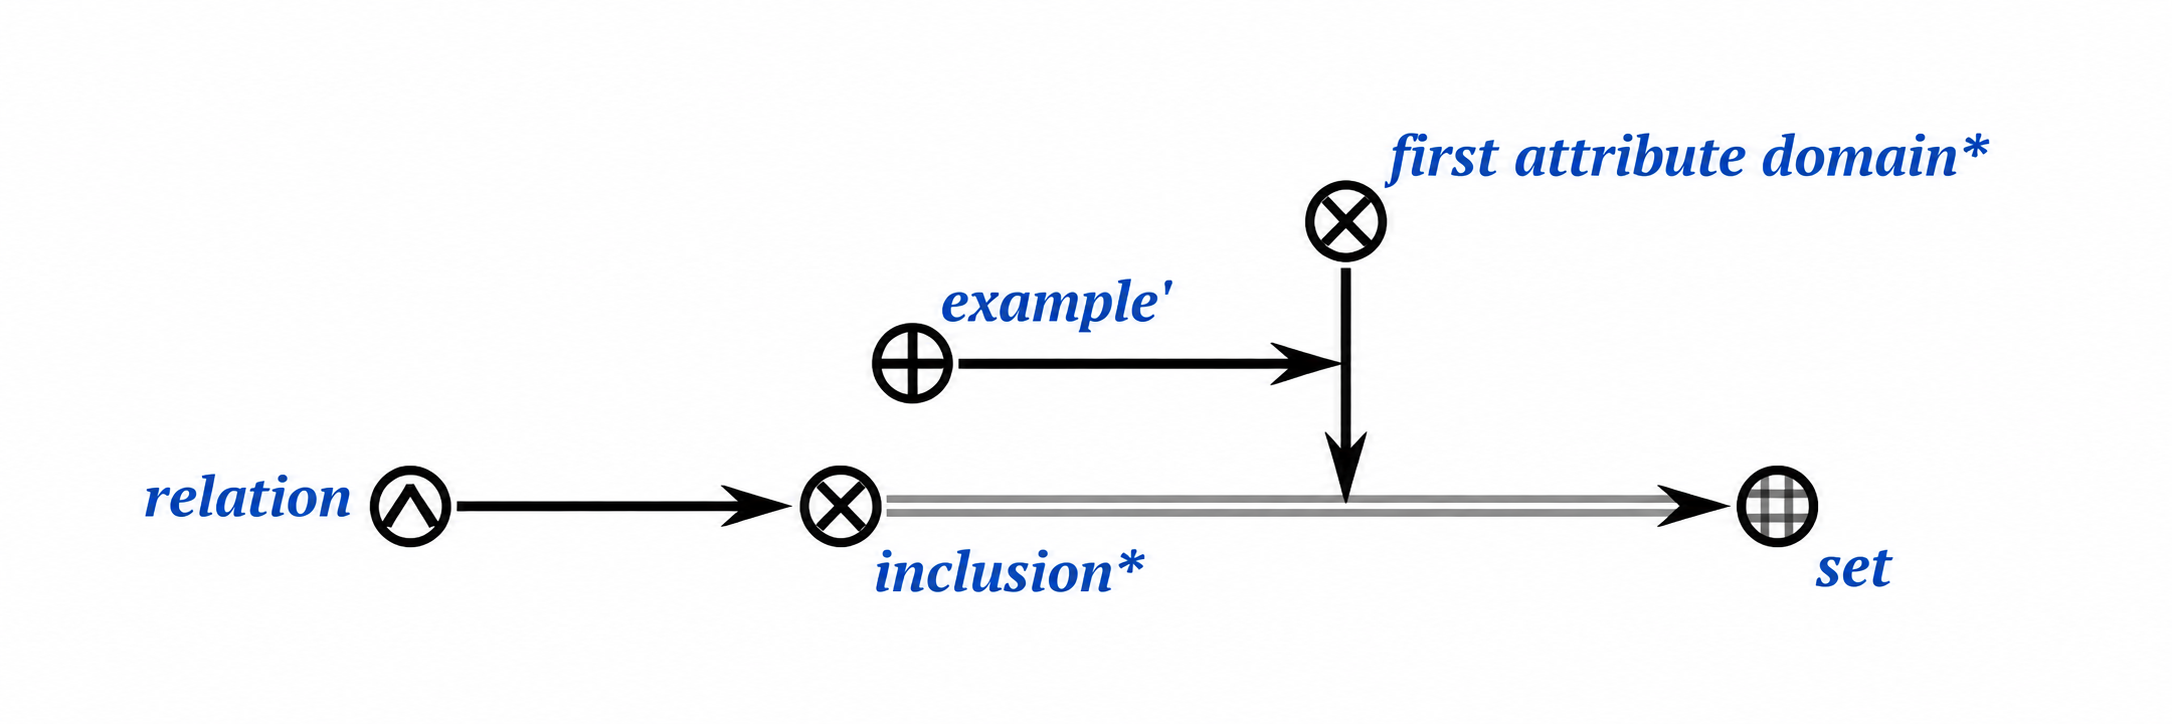
\includegraphics[height=89.25bp,keepaspectratio]{figures/sd_sets/firstDomen_en.png}
	\end{center}}
	\end{SCn}
\end{frame}

\begin{frame}{\\Second attribute domain}%
	\topline
	\justifying
	\begin{SCn}
	\scnheader{second attribute domain*}
	\scniselement{binary relation}
	\scntext{definition}{\textbf{\textit{second attribute domain*}} is a \textit{binary relation} that connects a relation to its domain for the attribute \textbf{\textit{2\scnrolesign}} of that relation.}
	\scnrelfrom{example description}{
		\begin{center}
		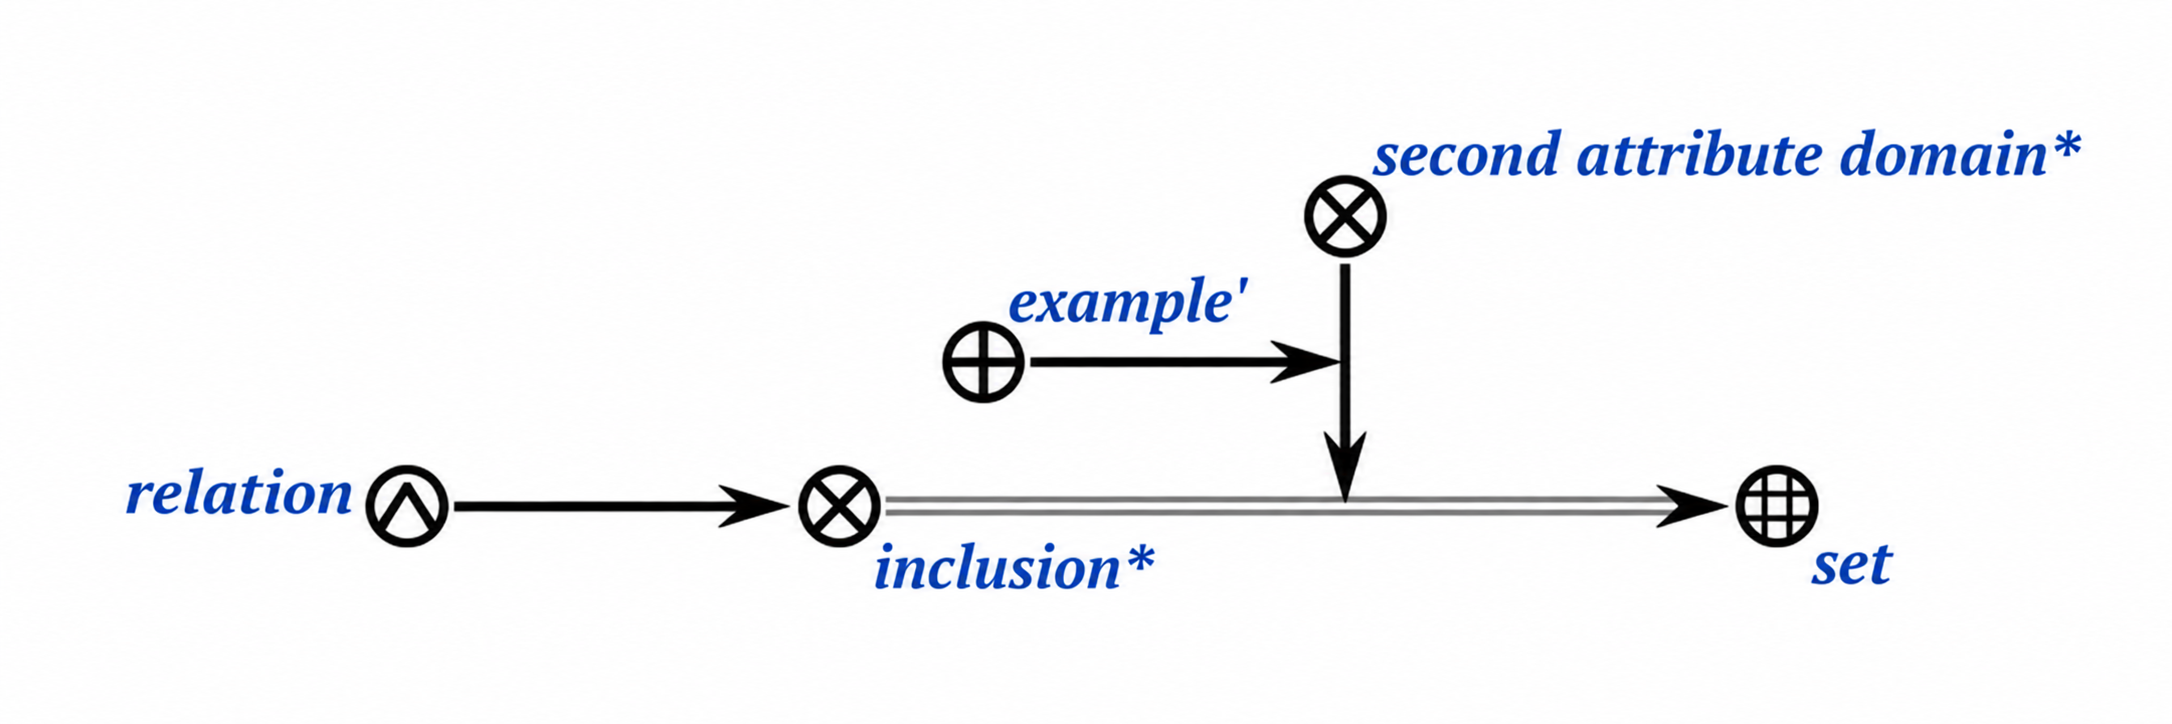
\includegraphics[height=89.25bp,keepaspectratio]{figures/sd_sets/secondDomen_en.png}
	\end{center}}
	\end{SCn}
\end{frame}

\begin{frame}{\\Composition of relations}%
	\topline
	\justifying
	\begin{SCn}
	\scnheader{composition of relations*}
	\scniselement{quasi-binary relation}

	\scntext{definition}{\textbf{\textit{composition of relations*}} is a \textit{quasi-binary relation} that connects two binary relations to their composition. The composition of binary relations \textbf{\textit{R}} and \textbf{\textit{S}} is defined as the set $\{(x, y) | \exists z(xSz \wedge zRy)\}$}
	\end{SCn}
\end{frame}

\begin{frame}%
	\scnrelfrom{example description}{
		\begin{center}
		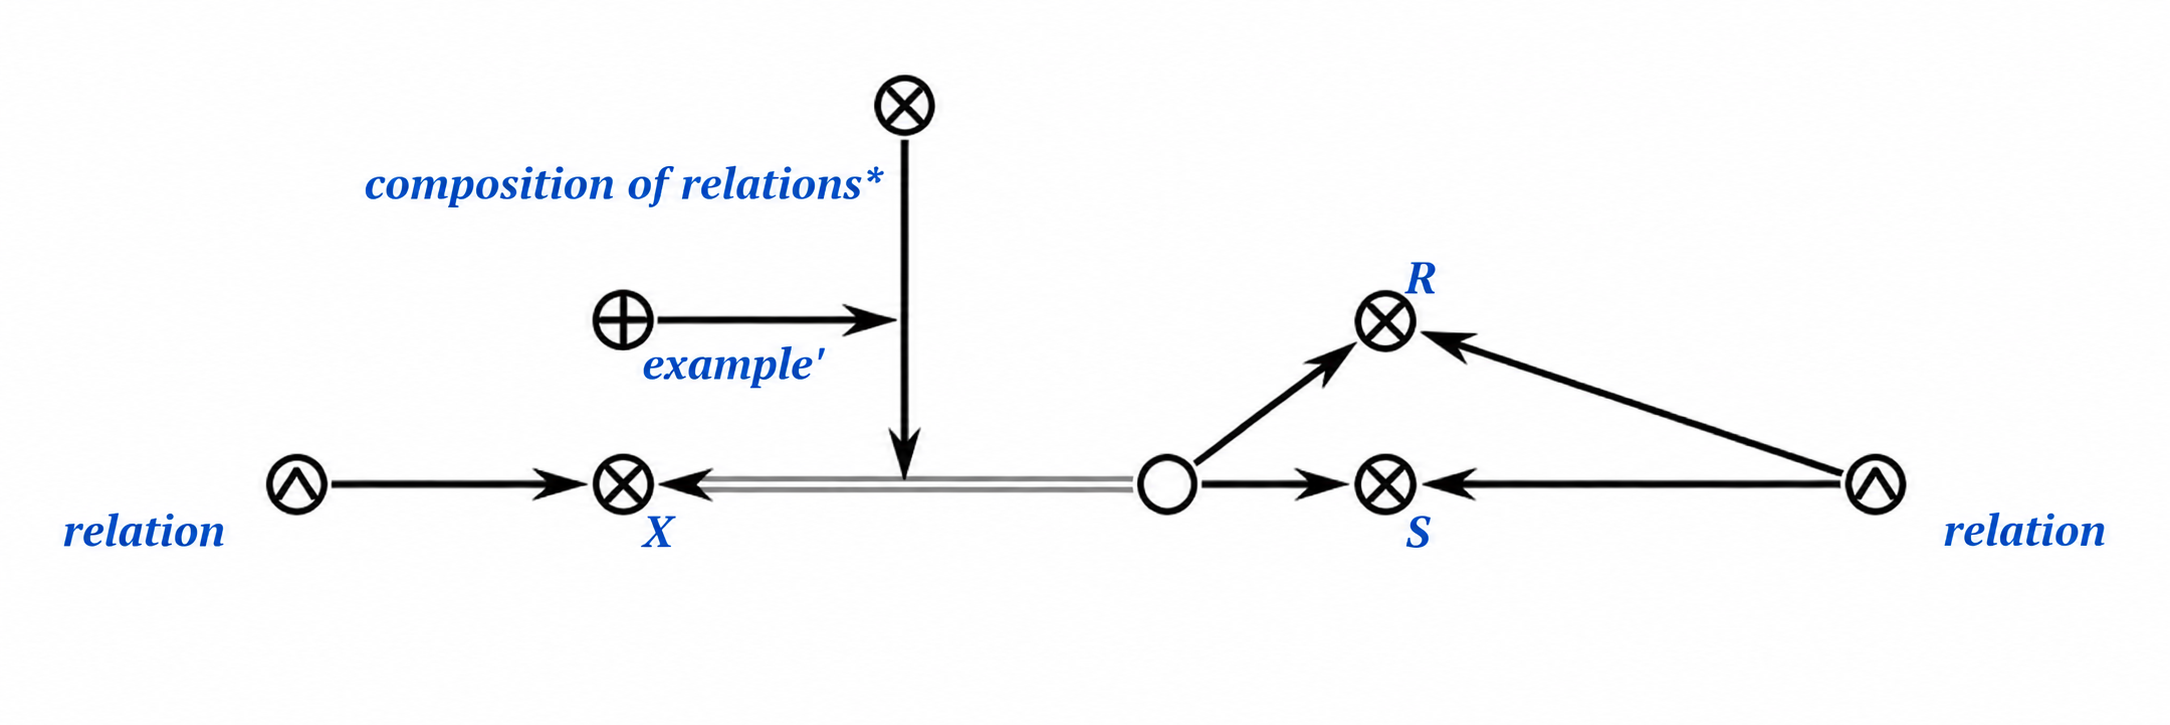
\includegraphics[width=120mm]{figures/sd_sets/relationshipComposition_en.png}
	\end{center}}
	\end{frame}

\begin{frame}{\\Quotient set}%
	\topline
	\justifying
	\begin{SCn}
		\scnheader{quotient set*}
		\scnidtf{be a quotient set*}
		\scnidtf{set of all maximal sets of pairwise equivalent elements*}
		\scnidtf{set of all equivalence classes for a given equivalence relation*}
		\scniselement{binary relation}

		\scntext{definition}{\textbf{\textit{quotient set*}} is a binary directed relation whose tuples connect an equivalence relation to the set of all its equivalence classes. Each such class is a maximal set of entities every pair of which belongs to that equivalence relation.}
	\end{SCn}
\end{frame}

\begin{frame}%
	\scnrelfrom{example description}{
	\begin{center}
		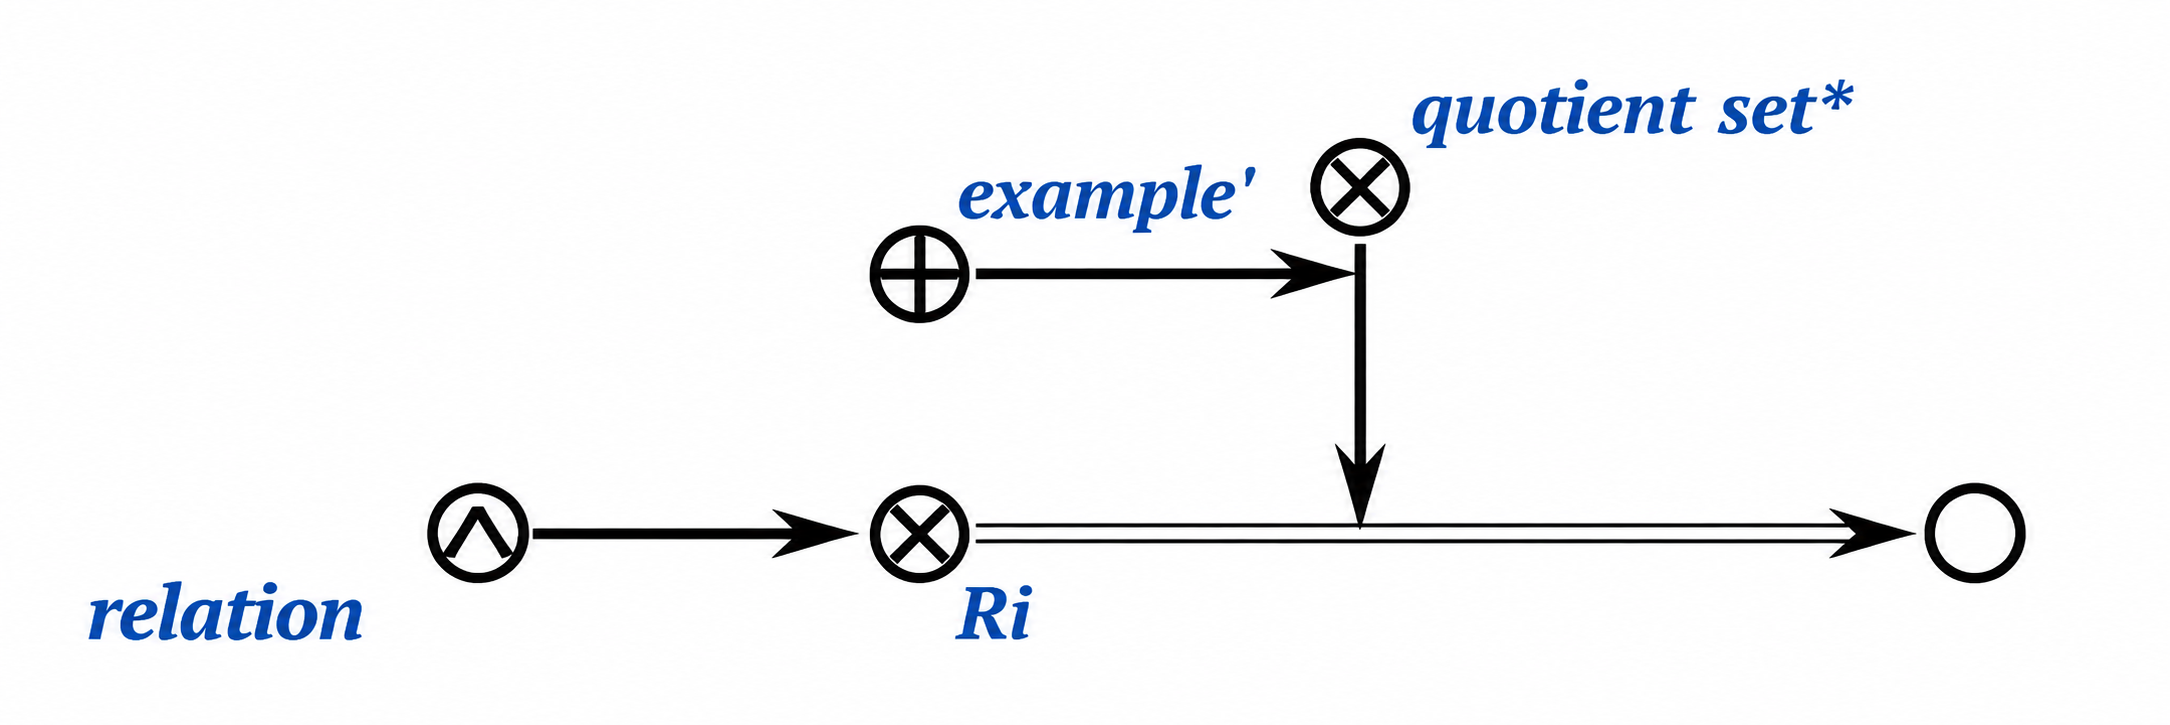
\includegraphics[width=80mm]{figures/sd_sets/factor_set_en.png}
	\end{center}}
\end{frame}

\begin{frame}{\\Metarelation}%
	\topline
	\justifying
	\begin{SCn}
		\scnheader{metarelation}
		\scntext{definition}{A metarelation is a \textit{relation} in each tuple of which at least one component is the sign of a \textit{relation}.}
		\scnhaselement{attribute domain*}
		\scnhaselement{attribute of a relation*}
		\scnhaselement{domain of definition*}
	\end{SCn}
\end{frame}
